\documentclass[a4paper, 11pt,            % impagina per fronte-retro
openright,               % inizio capitoli a destra                 
italian,
english                 
]{article}       %twoside

\usepackage[T1]{fontenc}
\usepackage[utf8]{inputenc}


\usepackage{listings}
\usepackage{color}
\usepackage{graphicx}
 \usepackage{float}
 
\definecolor{dkgreen}{rgb}{0,0.6,0}
\definecolor{gray}{rgb}{0.5,0.5,0.5}
\definecolor{mauve}{rgb}{0.58,0,0.82}

\lstset{frame=tb,
	language=Java,
	aboveskip=3mm,
	belowskip=3mm,
	showstringspaces=false,
	columns=flexible,
	basicstyle={\small\ttfamily},
	numbers=none,
	numberstyle=\tiny\color{gray},
	keywordstyle=\color{blue},
	commentstyle=\color{dkgreen},
	stringstyle=\color{mauve},
	breaklines=true,
	breakatwhitespace=true,
	tabsize=3
}

\setlength\parindent{0pt}


\begin{document}
	
		\section{L'ambiente Java: compilatore \& JVM}
	
	Java è compilato ad un bytecode intermedio a tempo di compilazione. Questo quindi è in contrasto con un linguaggio tipo C che viene compilato in codice macchina a tempo di compilazione. Il bytecode di Java non può essere eseguito direttamente sull'hardware, così come è possibile per C, deve invece essere interpretato dalla JVM a runtime per poter essere eseguito dall'hardware. Si può notare quindi come un linguaggio tipo C sia compilato solamente per una particolare architettura (quella su cui è stato compilato, ad esempio x86), non essendo quindi portabile. Ovviamente nulla toglie che potrebbe essere creato un hardware che implementi le specifiche della JVM: in questo caso il bytecode sarebbe eseguito direttamente sull'hardware, senza nessuno strato di interpretazione. Il Java bytecode infatti è un linguaggio macchina, soltanto che nel nostro caso viene è per la JVM.\\
	Essendo sia compilato che interpretato, Java porta con sé i pro e contro di queste due tipologie. \\
	\paragraph{L'interprete}
	L'interprete di Java è simile ad un dizionario: semplicemente per ogni istruzione bytecode guarda quale sia la corrispondente istruzione macchina e la manda da eseguire direttamente alla CPU. Se il codice viene eseguito più volte, il risultato sarà sempre lo stesso perchè le istruzioni non vengono analizzate e ottimizzate. \\
	\paragraph{Il compilatore}
	Il compilatore, a differenza dell'interprete, carica l'intero codice da eseguire a runtime. Man mano che lo traduce in bytecode, ha l'abilità di guardare a tutto o a pezzi del contesto runtime e prendere decisioni su come convertire il codice. Le sue decisioni sono basate sull'analisi di grafi di flusso creati dal codice come per esempio il prendere diversi branch o diversi dati a runtime.
	
	Quando una sequenza in bytecode è tradotta in codice macchina e possono essere eseguite delle ottimizzazioni, il set di istruzioni ottimizzato che è stato calcolato viene salvato su una struttura chiamata \textit{code cache}. La volta successiva che il bytecode viene eseguito, il codice ottimizzato precedentemente viene immediatamente trovato nella code cache e usato per l'esecuzione. In alcuni casi il compilatore può introdurre dei performance counter che servono per fare l'override delle precedenti ottimizzazioni e in quel caso il compilatore fa una nuova ottimizzazione sul codice. Il vantaggio della code cache è che l'instruction set risultante può essere eseguito direttamente senza nessuna compilazione o interpretazione, si salvano direttamente le istruzioni macchina. Questo velocizza di molto il tempo di esecuzione, soprattutto in Java che i metodi spesso vengono chiamati molte volte.
	
	
	
	
	\paragraph{JIT compiler}
	Tutte le implementazioni recenti della JVM hanno incorporato anche un compilatore just-in-time (JIT), cioè un compilatore interno, che al momento del lancio traduce al volo il programma bytecode Java in un normale programma nel linguaggio macchina del computer ospite. Questa ricompilazione è dinamica, cioè la macchina virtuale analizza costantemente il modello di esecuzione del codice e ottimizza ulteriormente le parti più frequentemente eseguite, mentre il programma è in esecuzione. Questo paga un prezzo in fase di lancio del programma, sebbene sia soltanto una piccola attesa. Le applicazioni Java risultanti però risultano decisamente più veloci e leggere. \\
	Nella fase di compilazione del bytecode è eseguita la maggior parte del "lavoro pesante", ovvero tutte quelle operazioni che richiedono molto tempo per essere eseguite, come l'analisi sintattica e semantica del codice sorgente e una prima fase di ottimizzazione; la compilazione da bytecode a codice nativo è invece molto più veloce.\\
	
	\paragraph{Ottimizzazione }
	Durante la compilazione dinamica vengono fatte delle ottimizzazioni. Queste possono essere fatto con dei performance counter. Ad esempio un performance counter che conta ogni volta che un blocco di bytecode viene chiamato (ad esempio un metodo specifico). Il compilatore utilizza queste informazioni su quanto "caldo" sia un blocco di codice per capire dove l'ottimizzazione potrà avere un miglior impatto sul programma. Il profiling a runtime permette al compilatore di fare moltissime ottimizzazioni a runtime. Su queste ottimizzazioni verranno fatte altre ottimizzazioni con l'avanzare del programma e così via.
	Un performance counter aumenta ogni volta che un metodo viene chiamato e noi impostiamo una soglia per dire "quando supera questa soglia voglio che parta l'ottimizzazione". Viene impostato con la flag TierXCompileThreshold=.
	
	Le soglie impostate sulla mia macchina sono queste:
	intx CompileThreshold                         = 10000                                  {pd product} {default}
	double CompileThresholdScaling                  = 1.000000                                  {product} {default}
	uintx IncreaseFirstTierCompileThresholdAt      = 50                                        {product} {default}
	intx Tier2CompileThreshold                    = 0                                         {product} {default}
	intx Tier3AOTCompileThreshold                 = 15000                                     {product} {default}
	intx Tier3CompileThreshold                    = 2000                                      {product} {default}
	intx Tier4CompileThreshold                    = 15000                                     {product} {default}
	
	
	
	
	
	
	
	
	Implementazioni della JVM:
	\begin{itemize}
		\item HotSpot. (con JIT)
	\end{itemize}
	
	Compilatori Java:
	\begin{itemize}
		\item javac: incluso nel JDK di Oracle;
		\item ECJ: compilatore di Eclipse
	\end{itemize}
	
	Tecniche per la performance della JVM HotSpot:
	\begin{center}
		https://wiki.openjdk.java.net/display/HotSpot/PerformanceTechniques
	\end{center}
	
	\subsection{OpenJDK}
	
	OpenJDK è il development kit gratis e open source, sviluppato da Sun microsystem dal 2006. È l'implementazione standard di riferimento da Java 7.
	
	Il JDK contiene diversi componenti: 
	\begin{itemize}
		\item JVM: HotSpot
		\item Java Class Library (JCL)
		\item Compilatore javac
	\end{itemize}
	
	Ciò che interessa a noi è la JVM HotSpot. HotSpot è formato da diversi componenti:
	
	\begin{itemize}
		\item un Java Classloader
		\item un Java bytecode interpreter
		\item Diversi garbage collectors
		\item Un set di librerie runtime di supporto
	\end{itemize}
	
	Esistono due diverse macchine virtuali disponibili: una versione Client e una versione Server. Si può decidere quale versione utilizzare semplicemente dando un'opzione a linea di comando. 
	
	\begin{itemize}
		\item \textbf{Client:} è una versione che è creata apposta per avere caricamenti rapidi. Non esegue molte ottimizzazioni e utilizza un interprete.È ottimizzato per essere molto più veloce allo start-up, in genere viene utilizzato per applicazioni client come le GUI. Perchè parte più veloce? perchè esegue molte meno delle ottimizzazioni complesse che richiede la versione server, richiedendo quindi molta meno memoria a runtime;
		\item \textbf{Server:} è una versione che carica più lentamente e consuma più risorse nell'ottimizzazione. Infatti produce codice più ottimizzato grazie a delle compilazioni JIT, per portare a performance migliori. È una versione che è progettata per eseguire applicazioni server che vengono eseguite per molto tempo, che devono avere una più alta velocità operativa possibile piuttosto che uno start-up veloce o un minor consumo di memoria. In particolare vengono eseguiti inlining, che sono costosi in memoria
		\item \textbf{Tiered:} la compilazione tiered combina la versione server e la versione client, unendo i vantaggi di entrambe. La prima volta è stata introdotta nella JVM Zing JVM di Azul. Da Java 7 è stata adottata da Oracle nella HotSpot JVM e da Java 8 è attiva di default. Il compilatore client è più attivo durante lo startup del programma e gestisce tutte le ottimizzazioni che sono gestite dai contatori di performance con le soglie più basse (ovvero che il codice è stato attraversato ancora poche volte). Inoltre questa versione client inserisce i performance counter nei punti più \textit{hot} e prepara set di istruzioni per le ottimizzazioni più avanzate, che verranno gestite successivamente dal compilatore server. La versione tiered è molto efficiente in termini di risorse poichè è capace di raccogliere dati durante le attività poco costose dal compilatore, che possono essere utilizzati per ottimizzazioni avanzate in seguito.
		
		Paragonato a codice solo interpretato, la versione client velocizza in generale un programma di 5-10 volte. La versione server invece guadagna 30-50\% e in molti casi il maggior dispendio di risorse è bilanciato dalle migliore performance. 
	\end{itemize}
	
	
	
	
	
	
	
	
	
	
	
	
	
	
	
	
	
	
	
	
	
	\section{Come fare benchmarking}
	Fare benchmarking non è facile: bisogna tenere conto di tutte le possibili ottimizzazioni della JVM. Benchmark fatti male possono farti credere che il tuo programma funzioni meglio di quello che lo sia in realtà.
	
	\subsection{Piattaforma}
	
	Utilizzo JMH, un framework per microbenchmarking per Java. Intanto per creare un progetto che utilizzi JMH bisogna creare un progetto Maven e impostare i vari parametri.
	Ho impostato come versione di Java la versione 8, quindi sia i test con gli stream sia i test per i for loop utilizzano la versione 8 di Java.
	
\begin{lstlisting}
import org.openjdk.jmh.annotations.Benchmark;

public class MyBenchmark {
	
	@Benchmark
	public void testMethod() {
		// This is a demo/sample template for building your JMH benchmarks. 
		// Put your benchmark code here.
		
		int a = 1;
		int b = 2;
		int sum = a + b;
	}
}
\end{lstlisting}

	Intanto bisogna creare dei benchmark come in questo esempio. Poi bisogna buildare il progetto con Maven e questo ci crea un file jar che potrà essere eseguito per far partire il benchmark.
	
	\subsection{Modalità di benchmark}
	
	I benchmark possono essere eseguiti in diversi modi. Possono essere scelti una o più di queste modalità:
	
	\begin{itemize}
		\item \textbf{Throughput: } Misura il numero di operazioni al secondo, ovvero il numero di volte al secondo che il benchmark può essere eseguito. 
		\item \textbf{Average Time: } Misura quanto tempo ci vuole per eseguire una singola esecuzione del metodo del benchmark. 
		\item \textbf{Sample Time: } Misura quanto tempo ci vuole per eseguire una singola esecuzione del metodo del benchmark, includendo il tempo minimo e massimo tra le iterazioni.
		\item \textbf{Single Shot Time: } Misura quanto tempo ci vuole per una singola esecuzione del metodo di un benchmark. Questo è utile per testare come performa un metodo su una partenza "da freddo", ovvero senza il warmup della JVM. 
		\item \textbf{All} Misura tutte quelle precedenti.
	\end{itemize}
	Bisogna scegliere una o più modalità e indicarle grazie a questa annotation:
	\begin{center}
		@BenchmarkMode({Mode.Throughput, Mode.AverageTime})
	\end{center}
	
	\subsection{Tempo di misurazione}
	È possibile indicare l'unità di tempo con cui verrà considerato il benchmark e verrà utilizzato da tutte le modalità del benchmark. Possono essere scelte queste unità temporali:
	\begin{itemize}
		\item NANOSECONDS
		\item MICROSECONDS
		\item MILLISECONDS
		\item SECONDS
		\item MINUTES
		\item HOURS
		\item DAYS
	\end{itemize}
	Bisogna scegliere una unità di tempo grazie a questa annotation: 
	\begin{center}
		@OutputTimeUnit(TimeUnit.MINUTES)
	\end{center}
	
	\subsection{Stato dei benchmark}
	È possibile inizializzare delle variabili che vengono utilizzate nel codice del benchmark, ma vogliamo che non siano parte del tempo di calcolo del benchmark. Queste variabili vengono chiamate "stati". Gli stati devono essere dichiarati in classi speciali e un'istanza di queste classi deve essere passata come parametro al metodo del benchmark. Le classi stato vengono annotate con @State.
	Un oggetto stato può essere utilizzato più volte dai metodi del benchmark. JMH prevede diversi scope dove questi oggetti possono essere riutilizzati e vengono indicati come parametri dell'annotazione @State.
	Possono esserci i seguenti scope:
	\begin{itemize}
		\item \textbf{Thread: } ogni thread che esegue il benchmark crea la propria istanza dell'oggetto
		\item \textbf{Group: } ogni gruppo di thread che esegue il benchmark crea la propria istanza dell'oggetto
		\item \textbf{Benchmark: } tutti i thread che eseguono il benchmark condividono lo stesso oggetto
	\end{itemize}
	Una classe deve avere queste caratteristiche per poter essere annotata con @State: 
	\begin{itemize}
		\item La classe deve essere public
		\item Se è una classe interna, deve essere dichiarata statica
		\item La classe deve avere un costruttore pubblico senza argomenti
	\end{itemize}
	
	È possibile aggiungere dei metodi alle classi stato che vengono invocati alla creazione dell'oggetto oppure quando viene concluso il benchmark. Questi metodi vengono aggiunti con l'annotazione @Setup e @Teardown.
	Il tempo di setup e teardown non è incluso nel tempo considerato dal benchmark. Si possono avere uno o più metodi di setup e teardown. Esempio:
	
	\begin{lstlisting}
	public class MyBenchmark {
		
		@State(Scope.Thread)
		public static class MyState {
		
		@Setup(Level.Trial)
		public void doSetup() {
			sum = 0;
			System.out.println("Do Setup");
		}
		
		@TearDown(Level.Trial)
		public void doTearDown() {
			System.out.println("Do TearDown");
		}
		
		public int a = 1;
		public int b = 2;
		public int sum ;
		}
		
		@Benchmark @BenchmarkMode(Mode.Throughput) @OutputTimeUnit(TimeUnit.MINUTES)
		public void testMethod(MyState state) {
			state.sum = state.a + state.b;
		}
	}
	\end{lstlisting}
	
	@Setup e @Teardown accettano dei parametri e possono essere di questi tre tipi: 
	\begin{itemize}
		\item \textbf{List.Trial:} il metodo viene chiamato solamente una volta per ogni esecuzione completa del benchmark. Con esecuzione completa si intende un "fork" completo, inclusi tutti i warmup e le iterazioni
		\item \textbf{List.Iteration:} il metodo viene invocato una volta per ogni iterazione del benchmark
		\item \textbf{List.Invocation:} il metodo viene invocato per ogni invocazione al metodo del benchmark
	\end{itemize}
	
	
	
	\section{Ottimizzazioni della JVM}
	
	Esistono delle ottimizzazioni della JVM che possono far sembrare il codice del benchmark molto più veloce di quanto lo sarebbe in un programma reale.
	
	\subsection{Eliminazione dead code}
	
	La JVM ottimizza il codice analizzando il cosiddetto \textit{dead code}, ovvero se la JVM vede che il risultato di una qualsiasi computazione non è mai utilizzato, lo considera \textit{dead code} e lo elimina.
	Il dead code include:
	\begin{itemize}
		\item Unreachable code;
		\item Codice che produce \textit{dead variables}, ovvero variabile scritte ma mai più lette.
	\end{itemize}

	Eliminare il dead code ha diversi vantaggi:
	\begin{itemize}
		\item Riduce il peso totale del programma;
		\item Fa evitare al programma di eseguire operazioni inutili, permettendo quindi di ridurre il tempo di esecuzione.
	\end{itemize}
	Ad esempio vediamo questo benchmark:
	
	\begin{lstlisting}
		public class MyBenchmark {
			@Benchmark
			public void testMethod() {
				int a = 1;
				int b = 2;
				int c = 3
				
				int sum = a + b;
			}
		}
	\end{lstlisting}
	
	La JVM opera quindi in questo modo:
	\begin{itemize}
		\item Vede che l'assegnazione c=3 assegna un valore a c ma non viene mai più letto, ovvero fa un'assegnazione ad una \textit{dead variable}. Poichè è una variabile locale ad una funzione, non può essere utilizzata al di fuori del proprio scope, e quindi viene eliminata;
		\item Vede che la computazione di a+b non è mai utilizzata e quindi la elimina;
		\item Vede quindi che la variabile sum non è utilizzata e quindi la elimina;
		\item Di conseguenza a e b non sono mai utilizzate (poichè non esiste più sum) e vengono di conseguenza eliminate anche loro.
	\end{itemize}
	Il risultato ottenuto è un metodo assolutamente vuoto e quindi un benchmark vuoto.
	
	Inoltre la JVM considera \textit{dead code} anche il codice irraggiungibile. Ad esempio in un benchmark dove si vuole testare un istruzione condizionale sempre falsa, l'intero blocco dell'if viene tolto a tempo di compilazione.
	Da notare l'assegnazione d = 4, ovvero l'assegnazione di un valore ad una variabile che non verrà mai usata. Questo fenomeno si chiama \textit{dead store}, ovvero scrittura su una variabile che non viene poi più letta. Ovviamente viene eliminata dalla JVM.
	
	\begin{lstlisting}
	public class MyBenchmark {
		@Benchmark
		public void testMethod() {
			int a = 1;
			int b = 2;
			int c;
			int d = 4;
			
			if (0)
				c=3;
			int sum = a + b;
		}
	}
	\end{lstlisting}
	
	Per finire bisogna notare che la maggior parte del dead code che viene eliminato, è il risultato di altre ottimizzazioni fatte dal compilatore più che di "distrazioni" del programmatore. Infatti man mano che vengono fatte delle ottimizzazioni, il codice si trova in una nuova forma che può essere analizzata a sua volta e continuare quindi ad applicare le regole. Il dead code aggiuntivo viene, ad esempio, creato dalla \textit{strength reduction}.
	
	\subsection{Evitare l'eliminazione del dead code}
	
	Per evitare la situazione descritta prima, bisogna modificare la funzione in un modo che faccia sembrare alla JVM che non ci sia dead code. Per farlo ci sono due modi:
	
	\begin{itemize}
		\item Ritornare il risultato della computazione del metodo del benchmark;
		\item Passare il risultato della computazione ad un \textit{black hole} fornito da JMH,
	\end{itemize}

	\textbf{Ritornare il valore da un metodo}
	\\
	
	\begin{lstlisting}
	public class MyBenchmark {
		@Benchmark
		public void testMethod() {
			int a = 1;
			int b = 2;
			int sum = a + b;
			
			return sum;
		}
	}
	\end{lstlisting}
	
	Adesso il metodo testMethod() ritorna il valore della variabile \textit{sum}. In questo modo la JVM non può eliminare l'addizione (a+b) poichè il valore di ritorno potrebbe essere utilizzato dal chiamante della funzione. JMH penserà di far credere alla JVM che il valore di ritorno sia effettivamente utilizzato dal chiamante e quindi la JVM non considera \textit{dead code}. Se JMH non facesse finta di utilizzare il valore ritornato dalla funzione, allora anche se ci fosse il return verrebbe considerato dead code (la JVM vede quando il valore di ritorno di una funzione è ignorato dal chiamante).\\
	
	Nel caso in cui si facciano computazioni su più variabili e si volessero ritornare quindi più variabili, basterà inglobarle all'interno di un unico elemento e ritornare quest'ultimo (ad esempio un oggetto con più campi dati, una lista ecc).
	
	\textbf{Passare il valore ad un \textit{black hole}}
	Un'alternativa a ritornare i valori calcolati nella funzione, è quella di utilizzare i \textit{black hole} di JMH. Vediamo un esempio:
	
	\begin{lstlisting}
		public class MyBenchmark {
			@Benchmark
			public void testMethod(Blackhole blackhole) {
				int a = 1;
				int b = 2;
				int sum = a + b;
				blackhole.consume(sum);
			}
		}
	\end{lstlisting}
	
	A differenza del metodo del "return", osserviamo che ora il benchmark vuole come parametro un oggetto di tipo \textit{Blackhole}. Questo oggetto verrà fornito direttamente da JMH quando invocherà il metodo per eseguire il benchmark. \\ 
	Il calcolo della funzione (a+b) ora, quindi, sarà passato al metodo \textit{consume} dell'istanza del Blackhole. Questo metodo farà credere alla JVM che la variabile \textit{sum} sia effettivamente utilizzata. \\
	Rispetto al metodo dei return è più comodo perchè nel caso il metodo utilizzi più variabili, basterà passare ciascuna di essere al Blackhole e non dover creare un oggetto che le inglobi.
	
	
	\subsection{Strength Reduction}
	La strength reduction è una tecnica di ottimizzazione nella quale il compilatore sostituisce delle operazioni costose (in termini computazionali) con delle operazioni equivalenti ma meno costose. Un classico esempio di questa tecnica è la conversione di moltiplicazioni all'interno di un ciclo con delle addizioni. Le addizioni tra interi sono più veloci delle moltiplicazioni in media di 3 volte.\\
	In aritmetica reale invece le moltiplicazioni potrebbero essere più veloci poiché:
	\begin{itemize}
		\item Le mantisse si moltiplicano tra loro 
		\item Si sommano gli esponenti delle mantisse
	\end{itemize}
	Queste operazioni possono essere svolte in parallelo.
	Mentre la somma tra due numeri reali, comporta queste operazioni:
	\begin{itemize}
		\item Normalizzazione della mantissa: shift della mantissa del primo numero in modo che il suo esponente sia uguale a quello del secondo numero;
		\item Somma delle due mantisse;
		\item La somma può andare in overflow di 1 bit e quindi il risultato deve essere normalizzato di nuovo
	\end{itemize}
	Questi step invece devono essere svolti in serie.\\
	Vediamo quindi un esempio di moltiplicazione che può essere sostituita da una addizione:
	\begin{lstlisting}
		c = 7;
		for (i = 0; i < N; i++){
			y[i] = c * i;
		}
	\end{lstlisting}
	Può essere sostituito da:
	\begin{lstlisting}
		c = 7;
		k = 0;
		for (i = 0; i < N; i++){
			y[i] = k;
			k = k + c;
		}
	\end{lstlisting}
	
	Osserviamo le operazioni assembly prima e dopo una strength reduction, per capire effettivamente quante istruzioni possono essere eliminate grazie a questa tecnica. Il codice in esame è il seguente:
	\begin{lstlisting}
		for (i = 0; i < n; i++){
			for (j = 0; j < n; j++){
				A[i,j] = 0.0;
			}
			A[i,i] = 1.0;
		}
	\end{lstlisting}
	Il compilatore vedrà questo codice come queste istruzioni:
	\begin{lstlisting}[language={[x86masm]Assembler}]
		0010  ; for (i = 0, i < n; i++)
		0020    {
		0030      r1 = #0                        ; i = 0
		0040  G0000:
		0050      load r2, n                     ; i < n
		0060      cmp r1, r2
		0070      bge G0001
		0080
		0090      ; for (j = 0; j < n; j++)
		0100        {
		0110           r3   = #0                 ; j = 0
		0120  G0002:
		0130           load r4, n                ; j < n
		0140           cmp r3, r4
		0150           bge G0003
		0160
		0170           ; A[i,j] = 0.0;
		0180           load r7, n
		0190           r8  = r1 * r7             ; calculate subscript i * n + j
		0200           r9  = r8 + r3
		0210           r10 = r9 * #8             ; calculate byte address
		0220           fr3 = #0.0
		0230           fstore fr3, A[r10]
		0240
		0250           r3 = r3 + #1              ; j++
		0260           br G0002
		0270        }
		0280  G0003:
		0290      ; A[i,i] = 1.0;
		0300      load r12, n                    ; calculate subscript i * n + i
		0310      r13 = r1 * r12
		0320      r14 = r13 + r1
		0330      r15 = r14 * #8                 ; calculate byte address
		0340      fr4 = #1.0
		0350      fstore fr4, A[r15]
		0360
		0370      ;i++
		0380      r1 = r1 + #1
		0390      br G0000
		0400    }
		0410  G0001:
	\end{lstlisting}
	
	Il compilatore in questo caso farà molte ottimizzazioni, non soltanto la strength reduction. Ad esempio le espressioni che sono invarianti all'interno di un ciclo possono essere tirate fuori dal ciclo. Molti registri possono essere uniti tra loro poichè alcune variabili non cambiano. Alla fine delle ottimizzazioni il codice si riduce a questo:
	\begin{lstlisting}[language={[x86masm]Assembler}]
	0115  ;       r9   = r8         killed
	0117           r20  = r8 + r2            ; limit
	0118           r10  = r8 * #8            ; initial value of r10
	0119           r22  = r20 * #8           ; new limit
	0120  G0002:
	0145  ;       cmp r9, r20       killed   ; r8 + j < r8 + n = r20
	0147           cmp r10, r22              ; r10 = 8*(r8 + j) < 8*(r8 + n) = r22
	0150           bge G0003
	0160
	0170           ; A[i,j] = 0.0;
	0230           fstore fr3, A[r10]
	0240
	0245           r10 = r10 + #8            ; strength reduced multiply
	0255  ;       r9 = r9 + #1      killed   ; loop variable
	0260           br G0002
	\end{lstlisting}
	
	Bisogna stare attenti anche a quando si vuole fare benchmark in cui si vogliono testare operazioni aritmetiche, perchè potrebbero essere più veloci di quanto si possa voler effettivamente testare.\\
	La strength reduction usa anche identità e proprietà matematica per sostituire operazioni matematiche lente con altre più veloci. Può infatti effettuare:
	\begin{itemize}
		\item Sostituzione di una divisione intera o moltiplicazione per una potenza di due, con uno shift aritmetico o logico;
		\item Sostituzione di una moltiplicazione per una costante con una combinazione di shift, addizione e sottrazioni;
		\item Sostituzione di una divisione intera con una moltiplicazione per una costante, traendo vantaggio dal numero limitato di bit per la rappresentazione degli interi.
	\end{itemize}
	
	Ad esempio:
	\begin{itemize}
		\item y = x / 8 diventa y = x >> 3
		\item y = x * 64 diventa y = x << 6
		\item y = x * 15 diventa y = (x << 4) - x
	\end{itemize}
	
	Quindi se l'obiettivo del benchmark è voler testare delle operazioni macchina (ad esempio testare l'overhead di moltiplicazione), è molto difficile riuscire nel proprio intento, proprio perchè la JVM ottimizzerà i calcoli in modo da non avere lo scenario "base" così come è stato scritto dal programmatore. 
	
	
	\subsection{Constant folding}
	
	Il constant folding è un'altra ottimizzazione del compilatore. Entra in gioco poichè un calcolo tra costanti risulta sempre uguale, anche se ripetuto più volte. La JVM rileva questo comportamento e quindi sostituisce il calcolo direttamente con il risultato del calcolo. Ad esempio, per l'espressione\\ 
	i = 300 * 250 * 45;\\ 
	non vengono generate due istruzioni di moltiplicazione e una di store. Invece viene calcolato il risultato dell'operazione a tempo di compilazione e sostituita la variabile direttamente con quel valore.
	Vediamo un esempio:
	
	\begin{lstlisting}
	public class MyBenchmark {
		@Benchmark
		public void testMethod() {
			int a = 1;
			int b = 2;
			int sum = a + b;
			
			return sum;
		}
	}
	\end{lstlisting}
	
	La JVM rileva che il valore di \textit{sum} è basato su due valori costanti (a e b). Può quindi sostituire il codice sopra con questo:
	
	\begin{lstlisting}
	public class MyBenchmark {
		@Benchmark
		public void testMethod() {
			int sum = 3;
			
			return sum;
		}
	}
	\end{lstlisting}
	
	Giunta a questa situazione, la JVM ritornerà direttamente 3, senza effettuare quindi l'allocazione della variabile in memoria.
	Come ulteriore passo di ottimizzazione inoltre, la JVM non chiamerà mai il metodo testMethod() poichè sa che ritornerà sempre 3 e sostituirà semplicemente la costante "3" dove c'era la chiamata al metodo.
	
	Nell'esempio di prima, prima di poter applicare il costant folding, si è dovuto applicare la \textit{constant propagation}, ovvero a tempo di compilazione vengono sostituite tutte le costanti note in tutte le espressioni. (ovvero a e b nell'esempio di prima).\\
	Vediamo un esempio dove viene utilizzata la constant propagation, constant folding, dead code elimination e infine una considerazione sulla sparse conditional constant propagation:
	
	\begin{lstlisting}
		int a = 30;
		int b = 9 - (a / 5);
		int c;
		
		c = b * 4;
		if (c > 10) {
			c = c - 10;
		}
		return c * (60 / a);
	\end{lstlisting}
	
	Applicando constant propagation seguita da costant folding diventa:
	
	\begin{lstlisting}
		int a = 30;
		int b = 3;
		int c;
		
		c = b * 4;
		if (c > 10) {
			c = c - 10;
		}
		return c * 2;
	\end{lstlisting}
	
	Ripetendo nuovamente due volte diventa:
	
	\begin{lstlisting}
		int a = 30;
		int b = 3;
		int c;
		
		c = 12;
		if (true) {
			c = 2;
		}
		return c * 2;
	\end{lstlisting}
	
	Ora a e b sono state sostituite ovunque nel loro scope e quindi può essere effettuata la dead code elimination:
	
	\begin{lstlisting}
		int c;
		c = 12;
		
		if (true) {
			c = 2;
		}
		return c * 2;
	\end{lstlisting}
	
	A questo punto potrebbe essere applicata anche la sparse conditional constant propagation, che selezionerebbe addirittura il branch appropriato in base alla condizione if. In questo caso il compilatore può vedere che l'if si valuta sempre a true, quindi il codice diventerebbe:
	
	\begin{lstlisting}
		return 4;
	\end{lstlisting}
	
	Per applicare questo tipo di ottimizzazione però il codice deve essere convertito in forma SSA (static single assignment form), ovvero una rappresentazione intermedia del codice che richiede che ogni variabile sia assegnata esattamente una volta ed ogni variabile sia definita prima di poter essere usata. Ho trovato che la JVM HotSpot utilizza una visione intermedia basata su SSA nel suo compilatore JIT.
	
	\subsection{Evitare il costant folding}
	
	Per evitare il costant folding bisogna evitare di inizializzare variabili esplicitamente. Invece è meglio utilizzare un'oggetto @State. In questo modo la JVM farà più fatica a riconoscere che i calcoli sono basati su costanti. Ad esempio:
	
	\begin{lstlisting}
	
	public class MyBenchmark {
		@State(Scope.Thread)
		public static class MyState {
			public int a = 1;
			public int b = 2;
		}
		
		@Benchmark 
		public int testMethod(MyState state) {
			int sum = state.a + state.b;
			return sum;
		}
	}
	\end{lstlisting}
	
	
	\subsection{Inlining}
	
	Molte ottimizzazioni cercano di eliminare le istruzioni macchina di jump poichè sono molto costose, poichè cambiano l'instruction pointer e cambiano il flusso d'esecuzione. Una delle più utili ottimizzazioni è l'inlining, ovvero fare l'inlining di alcune funzioni al posto di chiamarle. Se un metodo è chiamato molto spesso, quindi diventa un punto "hot", l'inlining può fare una grossa differenza. Inoltre dopo l'inlining spesso vengono applicate molte altre ottimizzazioni a catena. 
	
	
	
	











	\section{Ottimizzazione dei loop}
	
	Bisogna stare attenti ad usare i cicli all'interno del metodo del benchmark. Questo poichè la JVM è molto buona ad ottimizzare i cicli e quindi si possono avere risultati diversi da quelli che ci si aspetterebbe. Quindi non bisogna aggiungere un ciclo dove all'interno c'è effettivamente il corpo che si vuole testare, soltanto per farlo ripetere più volte e quindi evitare la chiamata al metodo del benchmark. Bisogna tenere i cicli soltanto se fanno effettivamente parte del nostro codice. \\
	Difficilmente uno stream potrà essere veloce come un ciclo for/while. Esistono infatti le seguenti ottimizzazioni per i cicli:
	\begin{itemize}
		\item Strength reduction;
		\item Induction variable analysis;
		\item Loop fission
		\item Loop fusion;
		\item Loop inversion;
		\item Loop interchange;
		\item Loop-invariant code motion;
		\item Loop nest optimization;
		\item Loop unrolling;
		\item Loop splitting;
		\item Loop unswitching;
		\item Software pipelining;
		\item Automatic parallelization.
	\end{itemize}

	
	\subsection{Loop fission}
	
	La loop fission è una ottimizzazione del compilatore in cui un loop è diviso in più loop, tutti con lo stesso range di indici, ma ognuno prende un pezzo del corpo del ciclo originale. L'obiettivo è quello di di suddividere un ciclo più grande in molti cicli più piccoli per utilizzare meglio la località dei dati. Questa suddivisione è molto più efficiente con processori multi core che possano assegnare ad ogni nuovo ciclo un processore a parte.
	
	
	
	
	\subsection{Loop fusion}
	
	La loop fusion è una ottimizzazione del compilatore che sostituisce diversi loop con uno singolo. Questo è possibile soltanto quando due cicli iterano sullo stesso range e non si riferiscono ai dati dell'altro. La loop fusion non sempre aumenta la velocità runtime di un programma. Infatti su alcune architetture due loop potrebbero andare più veloci di un singolo loop perchè viene utilizzata maggiormente la località dei dati. Vedere infatti \textit{Loop fission}
	
	\begin{lstlisting}
	int i, a[100], b[100];
	for (i = 0; i < 100; i++)
		a[i] = 1;                     
	for (i = 0; i < 100; i++)
		b[i] = 2;
	\end{lstlisting}
	
	può essere trasformato, ed è equivalente, a:
	
	\begin{lstlisting}
  	int i, a[100], b[100];
	for (i = 0; i < 100; i++){
		a[i] = 1; 
		b[i] = 2;
	}
	\end{lstlisting}
	
	\paragraph{Approfondimento località dei dati} la località dei dati avviene quando alcune zone di memoria sono accedute ripetutamente in un periodo di tempo breve. Ci sono due tipi di località di dati: temporale e spaziale. 
	\begin{itemize}
		\item \textbf{Temporale:} quando dati e risorse vengono richiesti entro un breve lasso temporale
		\item \textbf{Spaziale:} dati che sono stati immagazzinati in posizioni vicine nella memoria. Inoltre la località sequenziale accade quando gli elementi sono posizionati e acceduti in modo lineare, come un array monodimensionale.
	\end{itemize}
	Sistemi che utilizzano la cache sono ben disposti ad ottimizzazioni di questo tipo. 


	\subsection{Loop unrolling}
	È una tecnica di trasformazione di un ciclo che cerca di ottimizzare il tempo di esecuzione, a discapito della grandezza, in dimensioni, del codice sorgente. Può essere fatto manualmente o automaticamente dal compilatore. Il punto principale del loop unrolling è quello di aumentare la velocità di un programma riducendo o eliminando le istruzioni di controllo del ciclo, come le istruzioni per testare la fine di un ciclo ad ogni iterazione. Questo riduce il tempo che serve per fare un branch ogni volta, oltre a dover accedere ogni volta alle variabili dalla memoria. I cicli possono quindi essere riscritti come una sequenza ripetuta di statement simili. 
	
	\begin{figure}[H]
		\centering
		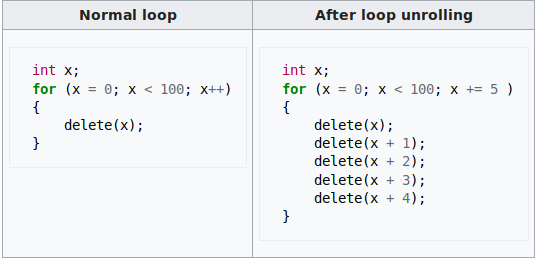
\includegraphics[width=10cm]{loop_unrolling.png}
	\end{figure}

	\begin{itemize}
		\item \textbf{Vantaggi:}
		\begin{itemize}
			\item Si eliminano moltissimi controlli a runtime se il compilatore è in grado di precalcolare gli offset individuali di tutte le variabili di un array, nel quale ci si riferisce con la variabile di controllo del ciclo. Le operazioni possono quindi direttamente essere scritte nel codice senza dover fare operazioni aritmetiche di puntatori a runtime
			\item È minimizzata la branch penalty, ovvero quando il branch predictor sbaglia a predirre se prendere un branch o meno. Infatti molti sistemi avanzati utilizzano un branch predictor che cerca di capire se il prossimo conditional jump verrà preso o meno. In quel caso mettono nella pipeline istruzioni ancora prima che il salto condizionali arrivi nella fase EXECUTE, risparmiando quindi cicli di clock. In caso poi la predizione fosse sbagliata, il lavoro in più viene scartato ma non ci si mette di più perchè è come se non si fosse fatta la predizione. 
			\item Se le istruzioni del ciclo sono indipendenti, si riesce a parallelizzare molto bene
		\end{itemize}
		\item\textbf{Svantaggi:}
		\begin{itemize}
			\item Aumento della grandezza del codice sorgente del programma, non voluto magari in applicazioni embedded
			\item Il codice diventa meno leggibile
			\item Se ci sono delle chiamate a funzioni dentro un loop, può diventare difficile fare l'inlining (ovvero sostituire il corpo della funzione con la chiamata), poichè la grandezza del codice potrebbe diventare eccessiva. 
		\end{itemize} 
	\end{itemize}


	\subsection{Loop unswitching}
	
	\begin{lstlisting}
	int i, w, x[1000], y[1000];
	for (i = 0; i < 1000; i++) {
		x[i] += y[i];
		if (w)
			y[i] = 0;
	}
	\end{lstlisting}
	
	
	diventa
	
	\begin{lstlisting}
	int i, w, x[1000], y[1000];
	if (w) {
		for (i = 0; i < 1000; i++) {
			x[i] += y[i];
			y[i] = 0;
		}
	} else {
		for (i = 0; i < 1000; i++) {
			x[i] += y[i];
		}
	}
	\end{lstlisting}
	
	
	
	
	
	
	

	
	
	\end{document} 
